\chapter{Food Chains}\label{ch:g3:food-chains}

Grass grows in the meadow. A grasshopper eats the grass. A
lizard catches the grasshopper. A buzzard, circling high, takes
the lizard. Four meals --- and suddenly the buzzard's afternoon
depends on how green the grass grew. \omterm{def:g2:caring-for-nature:environment}{Nature}'s meals link up
into chains, and learning to read them is learning how a whole
meadow holds together.

\section{Reading and writing a food chain}

\begin{definition}[Food chain]\label{def:g3:food-chains:chain}
A \emph{food chain}\index{food chain} is a line of \omterm{def:g1:living-or-not:living}{living
things} in which each one is eaten by the next. It is written
with arrows, each arrow meaning \emph{``is eaten
by''}\index{is eaten by}:
\[
\text{grass} \longrightarrow \text{grasshopper}
\longrightarrow \text{lizard} \longrightarrow \text{buzzard}.
\]
Each \omterm{def:g1:living-or-not:living}{living thing} is a \emph{link}\index{link} of the chain.
\end{definition}

\begin{remark}[Mind the arrow's direction]\label{rem:g3:food-chains:arrow}
The arrow points from the eaten to the eater --- it follows the
food. ``Grass $\rightarrow$ grasshopper'' reads ``grass \omterm{def:g3:food-chains:chain}{is
eaten by} the grasshopper''. Writing the arrows backward ---
toward the meal --- is the commonest mistake in \omterm{def:g3:food-chains:chain}{food chains};
remember that the arrow shows where the food \emph{goes}.
\end{remark}

\begin{proposition}[Every chain starts with a plant]\label{prop:g3:food-chains:start}
The first link of a \omterm{def:g3:food-chains:chain}{food chain} is always a \omterm{def:g1:plants-around-us:plant}{plant} (or another
\omterm{def:g1:living-or-not:living}{living thing} that makes its own food). \omterm{def:g1:plants-around-us:plant}{Plants} alone feed
without eating anyone --- from light, water and air, as
\cref{def:g1:plants-around-us:plant} said. Every \omterm{def:g1:animals-around-us:animal}{animal} link
lives, directly or through others, on that first green link.
\end{proposition}
\admitted

\begin{example}[Chains from three habitats]\label{ex:g3:food-chains:three}
In the pond: water \omterm{def:g1:plants-around-us:plant}{plants} $\rightarrow$ tadpole $\rightarrow$
dragonfly larva $\rightarrow$ stickleback $\rightarrow$ heron.
In the forest: oak \omterm{def:g1:plants-around-us:parts}{leaves} $\rightarrow$ \omterm{ex:g2:animals-grow-up:butterfly}{caterpillar}
$\rightarrow$ blue tit $\rightarrow$ sparrowhawk. In the
garden: salad $\rightarrow$ snail $\rightarrow$ hedgehog. First
link: always green.
\end{example}

\begin{omfigure}
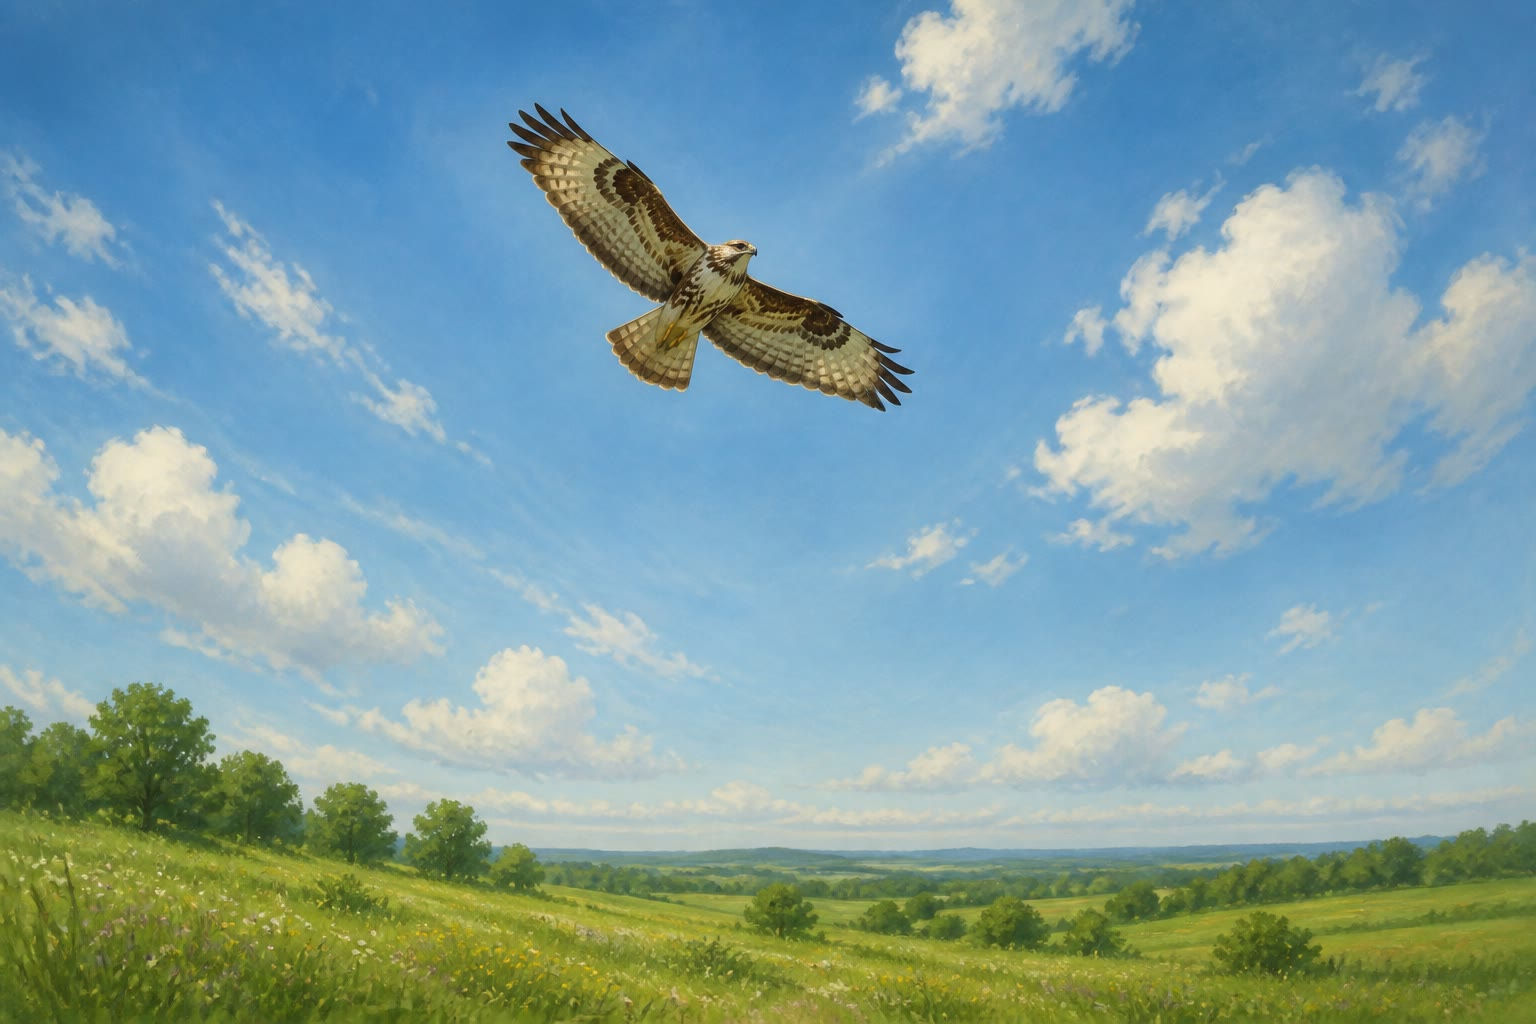
\includegraphics[width=0.6\linewidth]{images/book1/ai/g3-chains-buzzard.jpg}

{\small The meadow chain's last link on patrol: the buzzard's
afternoon depends, three links down, on how green the grass
grew.}
\end{omfigure}

\begin{method}[Building a food chain]\label{met:g3:food-chains:build}
\begin{enumerate}
  \item Choose an \omterm{def:g1:animals-around-us:animal}{animal} and ask: what does it eat? Write the
        food to its left, arrow pointing at the eater;
  \item ask the same question of the food, and continue leftward
        until you reach a \omterm{def:g1:plants-around-us:plant}{plant};
  \item ask: who eats my starting \omterm{def:g1:animals-around-us:animal}{animal}? Extend rightward while
        there is an eater;
  \item check every arrow reads \omterm{def:g3:food-chains:chain}{``is eaten by''} --- food flowing
        to the right.
\end{enumerate}
\end{method}

\section{When a link changes}

\begin{proposition}[Links depend on each other]\label{prop:g3:food-chains:depend}
In a \omterm{def:g3:food-chains:chain}{food chain}, every link depends on the ones before it, and
feeds the ones after it. If one link becomes scarce, the next
links go hungry --- and the link \emph{before} it, no longer
eaten so much, may multiply. A change in one link travels along
the whole chain.
\end{proposition}
\admitted

\begin{example}[The dry summer]\label{ex:g3:food-chains:dry}
A drought browns the meadow grass. Grasshoppers, short of food,
grow few; the lizards that hunted them go hungry and feed the
buzzard poorly in their turn. One brown first link, and the
whole chain above it thins --- the buzzard never ate grass, yet
it feels the drought.
\end{example}

\begin{example}[Removing the hunter]\label{ex:g3:food-chains:hunter}
Suppose the buzzards vanish from the valley. Lizards, less
hunted, multiply; grasshoppers are then eaten harder and
dwindle; the grass, less nibbled, may even thicken. Removing
the \emph{last} link also travels down the chain --- in the
other direction.
\end{example}

\begin{remark}[Real meadows are webs]\label{rem:g3:food-chains:web}
Our chain is a single thread, but the buzzard also takes mice,
the lizard also eats flies, and the grass feeds rabbits too.
Many chains crossing make a net --- the \emph{food web} that a
later year will study
(\cref{ch:g2:what-animals-eat} already hinted at it with the
fox, the rabbit and the grass). Chains first: they are the
threads the net is woven from.
\end{remark}

\section{Exercises}

\begin{exercise}[$\star$]\label{exo:g3:food-chains:1}
What does the arrow of a \omterm{def:g3:food-chains:chain}{food chain} mean? Which way does it
point?
\end{exercise}

\begin{exercise}[$\star$]\label{exo:g3:food-chains:2}
What kind of \omterm{def:g1:living-or-not:living}{living thing} is always the first link? Why?
\end{exercise}

\begin{exercise}[$\star$]\label{exo:g3:food-chains:3}
Write the meadow chain of this chapter with its four links and
its arrows.
\end{exercise}

\begin{exercise}[$\star$]\label{exo:g3:food-chains:4}
Correct this chain: fox $\rightarrow$ rabbit $\rightarrow$
grass.
\end{exercise}

\begin{exercise}[$\star$]\label{exo:g3:food-chains:5}
Build a chain from these links: blue tit, oak \omterm{def:g1:plants-around-us:parts}{leaves},
sparrowhawk, \omterm{ex:g2:animals-grow-up:butterfly}{caterpillar}.
\end{exercise}

\begin{exercise}[$\star$]\label{exo:g3:food-chains:6}
In the garden chain salad $\rightarrow$ snail $\rightarrow$
hedgehog, who \omterm{def:g3:food-chains:chain}{is eaten by} the snail? Who eats the snail?
\end{exercise}

\begin{exercise}[$\star$]\label{exo:g3:food-chains:7}
Use \cref{met:g3:food-chains:build} to make a chain of at least
three links ending with the heron of the pond.
\end{exercise}

\begin{exercise}[$\star$]\label{exo:g3:food-chains:8}
In the dry summer of \cref{ex:g3:food-chains:dry}, why does the
buzzard suffer although it never eats grass?
\end{exercise}

\begin{exercise}[$\star\star$]\label{exo:g3:food-chains:9}
Gardeners who poison every snail sometimes lose their hedgehog
--- and then meet \emph{more} slugs and snails than before.
Explain both halves with
\cref{prop:g3:food-chains:depend}.
\end{exercise}

\begin{exercise}[$\star\star$]\label{exo:g3:food-chains:10}
``The lizard depends on the grass.'' True or false? Defend your
answer with the meadow chain --- and say in which direction a
grass failure travels.
\end{exercise}
